\begin{figure}
  \centering
  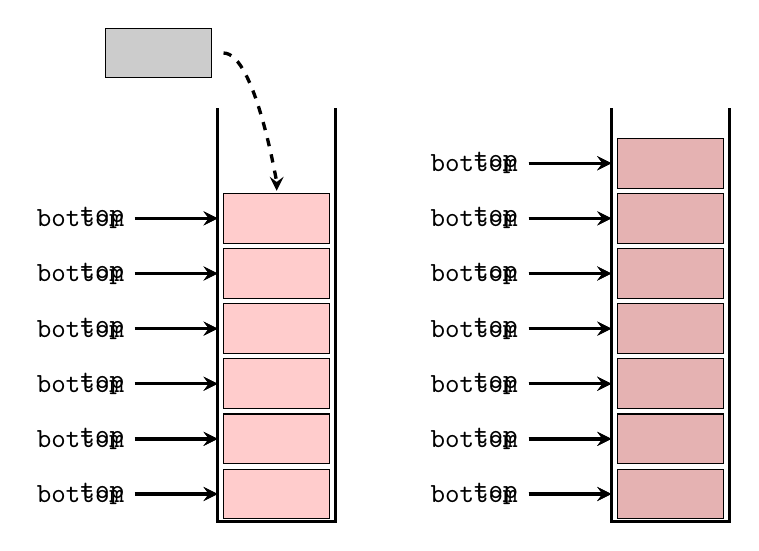
\begin{tikzpicture}
    \tikzstyle{information text}=[rounded corners,fill=blue!20,inner sep=1ex]

    \def\x{1.5}
    \def\y{0.7}
    \def\r{0.5}
    \def\c{9}
    
    \filldraw[fill=black!40,fill opacity=0.5] (\r+0.05*\x,\c*\y-0.95*\y)rectangle(\r+0.95*\x,\c*\y-0.05*\y); 
    \draw[->,>=stealth,dashed,very thick] (\r+1.05*\x,\c*\y-0.5*\y) .. controls +(right:4mm) and +(up:1mm) .. (2+0.5*\x,6*\y);

    \def\r{2}
    \draw[very thick] (\r,7.5*\y)--(\r,0*\y)--(\r+\x,0*\y)--(\r+\x,7.5*\y);
    \foreach \c in {1,2,...,6}{
      \filldraw[fill=red!40,fill opacity=0.5] (\r+0.05*\x,\c*\y-0.95*\y)rectangle(\r+0.95*\x,\c*\y-0.05*\y);
      \ifthenelse{\c=1}{
        \draw[->,>=stealth,very thick] (\r-0.7*\x,\c*\y-0.5*\y) node[left] {\tt{bottom}}--(\r+0,\c*\y-0.5*\y);
      }{}
      \ifthenelse{\c=6}{
        \draw[->,>=stealth,very thick] (\r-0.7*\x,\c*\y-0.5*\y) node[left] {\tt{top}}--(\r+0,\c*\y-0.5*\y);
      }{}
    }

    \pause 
    \def\r{7}
    \draw[very thick] (\r,7.5*\y)--(\r,0*\y)--(\r+\x,0*\y)--(\r+\x,7.5*\y);
    \foreach \c in {1,2,...,7}{
      \ifthenelse{\c=7}{
        \filldraw[fill=black!40,fill opacity=0.5] (\r+0.05*\x,\c*\y-0.95*\y)rectangle(\r+0.95*\x,\c*\y-0.05*\y);
        \draw[->,>=stealth,very thick] (\r-0.7*\x,\c*\y-0.5*\y) node[left] {\tt{top}}--(\r+0,\c*\y-0.5*\y);
      }{
        \filldraw[fill=red!40,fill opacity=0.5] (\r+0.05*\x,\c*\y-0.95*\y)rectangle(\r+0.95*\x,\c*\y-0.05*\y);
      }
      
      \ifthenelse{\c=1}{
        \draw[->,>=stealth,very thick] (\r-0.7*\x,\c*\y-0.5*\y) node[left] {\tt{bottom}}--(\r+0,\c*\y-0.5*\y);
      }{}
      
    }
  \end{tikzpicture}
  \caption{进栈}
\end{figure}
